\documentclass[a4paper,12pt]{article} % тип документа
\usepackage[margin=1in]{geometry} % Поля

%  Русский язык
\usepackage[warn]{mathtext}
\usepackage[T2A]{fontenc}			% кодировка
\usepackage[utf8]{inputenc}			% кодировка исходного текста
\usepackage[english,russian]{babel}	% локализация и переносы
% Математика
\usepackage{amsmath,amsfonts,amssymb,amsthm,mathtools} 
\usepackage{wasysym}
%%%
\usepackage{graphicx}

\usepackage{tabularx}

\usepackage{gensymb} % знак градуса
\usepackage{enumitem} % изменить список enumerate
\usepackage{placeins} % \FloatBarrier

\renewcommand{\thesection}{\Roman{section}} 
\renewcommand{\thesubsection}{\roman{subsection}}


\begin{document}

\newcolumntype{Y}{>{\centering\arraybackslash}X} %new tabularx


%титул
\hrule 	
\medskip
\begin{raggedright}
{\large \textbf{Отчёт по работе 4.3.3}}
\\
\medskip
{\Large Изучение разрешающей способности микроскопа методом Аббе} 
\\
\medskip
{\large Карташов Констанин Б04-005}
\medskip
\hrule
\medskip
\end{raggedright}


\section{Анотация}

\paragraph{Цель работы:} 
Определение дифракционного предела разрешения объектива микроскопа методом Аббе.

\paragraph{Оборудование:}
\begin{itemize}
\renewcommand{\labelitemi}{$\triangleright$}
\itemsep0em
\item Лазер
\item Кассета с набором сеток разного периода
\item Линзы
\item Щель с микрометрическим винтом
\item Экран
\item Линейка
\end{itemize}


\medskip\hrule\medskip
\FloatBarrier

\section{Теоретическая часть}

\subsection{Устройство экспериментальной установки}

\begin{figure}
\centering
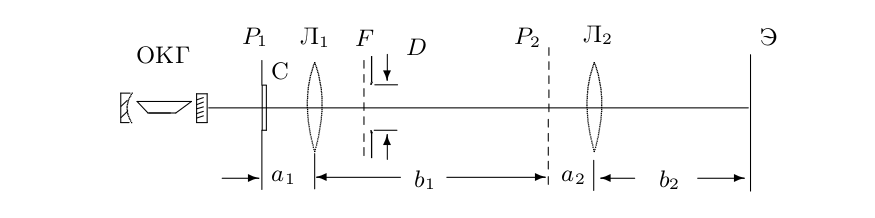
\includegraphics[width=\textwidth]{setup.png}
\caption{Схема экспериментальной установки -- модель проекционного микроскопа}
\label{fig:setup}
\end{figure}

\paragraph{} Экспериментальная установки представляет из себя модель проекционного микроскопа с длиннофокусной линзой Л$_1$  и короткофокусной линзой Л$_2$ с фокусными расстояниями $F_1 = 110$ мм и $F_1 = 25$ мм соответственно. 

\paragraph{} На расстоянии $a_1$ от длиннофокусной линзы расположена кассета с дифракционными сетками, а в её внутренней фокальной плоскости расположена щель. На расстоянии $b_2$ от короткофокусной линзы расположен экран.

\subsection{Разрешающая способность}

\begin{figure}
\centering
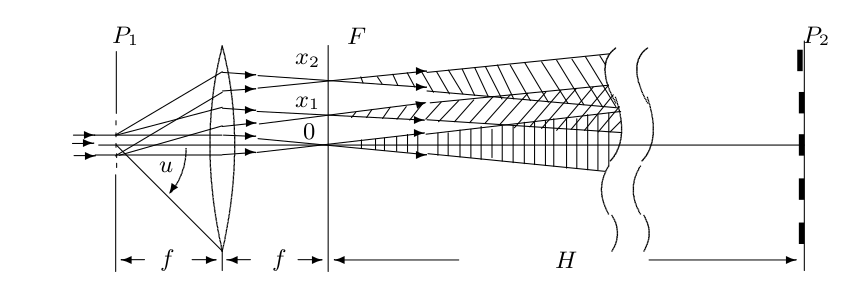
\includegraphics[width=\textwidth]{image.png}
\caption{Образование изображения в объективе микроскопа}
\label{fig:image}
\end{figure}

\paragraph{} Согласно теории Аббе минимальное разрешаемое объективом расстояние определяется условием:

\begin{equation}
l_{\min{}} \approx \frac{\lambda}{\sin A} \approx \frac{\lambda}{D / 2f},
\label{e:abbe}
\end{equation}

\noindent где $D$ -- диаметр диафрагмы. При этом диафрагма, расположенная симметрично, пропускает нулевой и $\pm 1$ дифракционные максимумы.

\medskip\hrule\medskip

\section{Экспериментальная часть}

\subsection{Измерение периодов решёток по их пространственному спектру}

\paragraph{} Поставим кассету с пятью дифракционными решётками на оптический стол, на расстоянии $H$ от экрана. Измеряя расстояние $L_n$ между $n$ максимумами определим расстояние $L$ между соседними для каждой решётке, затем вычислим дифракционный угол $\theta$, и период каждой решётки.

\begin{equation}
\theta = \frac{L_n}{(n - 1) H}, \;\;\; d = \frac{\lambda}{\theta} = \frac{\lambda H (n - 1)}{L_n}
\label{e:period}
\end{equation}


\paragraph{} Измерим расстояние $H$ при помощи линейки и отметки <<120 см>> на столе, получим: $H = 139$ см. Так как невозможно точно измерить положение сетки в кассете, будем считать погрешность примерно равной толщине кассеты, итого $H = 139 \pm 1$ см.

\paragraph{} При измерении расстояния между максимумами учтём погрешность линейки ($0.5$ мм) и толщину пятна $\Delta \approx 4$ мм. Так толщина пятна в восемь раз больше погрешности линейки, будем считать погрешность измерений $\sigma_L = \Delta / 2 \cdot \sqrt{2} \approx 3$ мм (два пятная с разных концов).

\paragraph{} Погрешность измерения периода, по формуле (\ref{e:period}):

\[
\sigma_d = d \cdot \sqrt{\left( \frac{\sigma_L}{L_n} \right) ^ 2 + \left( \frac{\sigma_H}{H} \right) ^ 2} = d \cdot \sqrt{\left( \frac{3 \text{ мм}}{L_n} \right) ^ 2 + 5 \cdot 10^{-5}}
\]

\paragraph{} Данные измерений и вычислений запишем в таблицу \ref{tab:1met}.

\begin{table}[]
\centering
\begin{tabular}{|l|l|l|l|l|l|l|}
\hline
$N$ & $n$ & $L_n$, мм & $L$,  мм & $\theta$, рад & $d$, мкм & $\sigma_d$, мкм \\ \hline
1   & 7   & 223       & 37.2     & 0.0267        & 19.90    & 0.30            \\ \hline
2   & 9   & 197       & 24.6     & 0.0177        & 30.03    & 0.50            \\ \hline
3   & 17  & 198       & 12.4     & 0.00890       & 59.8     & 1.0             \\ \hline
4   & 29  & 173       & 6.2      & 0.00445       & 119.7    & 2.2             \\ \hline
5   & 46  & 207       & 4.6      & 0.00331       & 160.8    & 2.6             \\ \hline
\end{tabular}
\caption{Данные для первого метода}
\label{tab:1met}
\end{table}

\subsection{Определение периода решёток по изображению, увеличенному с помощью микроскопа}

\paragraph{} Соберём модель проекционного микроскопа в соответствии с рис. \ref{fig:setup} из длиннофокусный линзы ($F_1 = 110$ мм) и короткофокусной линзы ($F_2 = 25$ мм). Определим расстояния $a_1, a_2, b_1, b_2$:

\[
a_1 = 14 \text{ см}, \; a_2 = 2.5 \text{ см}, \; b_1 = 84.5 \text{ см}, \; b_2 = 40 \text{ см}.
\]

\noindent Увеличение микроскопа рассчитаем как произведение увеличения двух линз:

\begin{equation}
\Gamma = \frac{b_1 b_2}{a_1 a_2} = \frac{84.5 \cdot 40}{14 \cdot 2.5} \approx 97.
\label{e:mag}
\end{equation}

\noindent Так как определить точное расстояние между центрами линз из-за широкой оправы, будем считать погрешность измерения расстояний по ширине оправы $\sigma_L \approx 1$ см, $a_2$ берём без погрешности, так как считаем его равным фокусному расстоянию $F_2$. Рассчитаем погрешность значения увеличения исходя из формулы (\ref{e:mag}):

\[
\sigma_\Gamma = \Gamma \cdot \sqrt{\left( \frac{\sigma_L}{b_1} \right) ^ 2 + \left( \frac{\sigma_L}{b_2} \right) ^ 2 + \left( \frac{\sigma_L}{a_1} \right) ^ 2} \approx 7
\]

\paragraph{} Для каждой дифракционной решётки получим её увеличенное изображение. Заметим, что полученное изображение искажено по краям, это связанно с геометрией линзы. В пределах мало искажённого участка изображения ($\approx \pm 5$ см от оптической оси) измерим расстояние $L_n$ между краями $n$ клеток, и ширину решётки $\delta L$. Рассчитаем период решётки и погрешность по формуле:

\[
d = \frac{L_n}{n \Gamma}, \;\;\; \sigma_d = d \cdot \sqrt{\left( \frac{\sigma_L}{L_n} \right) ^ 2 + \left( \frac{\sigma_\Gamma}{\Gamma} \right) ^ 2 } = d \cdot \sqrt{\left( \frac{\sigma_L}{L_n} \right) ^ 2 + 5 \cdot 10^{-3} }.
\]

\noindent В качестве погрешности $\sigma_L$ возьмём значения $\delta L$ так как они больше погрешности линейки, кроме случая для первой решётки. Результаты измерений и вычислений запишем в таблицу \ref{tab:2met}.

\begin{table}[]
\centering
\begin{tabular}{|l|l|l|l|l|l|l|}
\hline
$N$ & $n$ & $L_n$, мм & $\delta L$,  мм & $L$, мм & $d$, мкм & $\sigma_d$, мкм \\ \hline
1   & 30  & 44        & ?              & 1.5     & 15.2     & 1.1             \\ \hline
2   & 30  & 65        & 1              & 2.2     & 22.4     & 1.6             \\ \hline
3   & 15  & 101       & 1              & 6.7     & 69.7     & 5.0             \\ \hline
4   & 6   & 79        & 3              & 13.2    & 136      & 11              \\ \hline
5   & 6   & 102       & 4              & 17.0    & 176      & 14              \\ \hline
\end{tabular}
\caption{Данные для второго метода}
\label{tab:2met}
\end{table}

\subsection{Определение периодов микроскопа по оценке разрешающей способности микроскопа}

\paragraph{} Расположим в фокальной плоскости длиннофокусной линзы диафрагму в соответствии с рис. \ref{fig:setup}. Для каждой решётки определим минимальный размер диафрагмы $D$, при котором ещё различима картинка сетки. По формуле (\ref{e:abbe}) вычислим период решётки. Оценить точность такого метода сложно так, как превращение изображение сетки в изображение полос происходит плавно, и для разных решёток оно происходит с разной скоростью. Результаты измерений и вычислений запишем в таблицу \ref{tab:3met}.

\begin{table}[]
\centering
\begin{tabular}{|l|l|l|}
\hline
$N$ & $D$, мкм & $d$, мкм \\ \hline
1   & ?        & ?        \\ \hline
2   & 3300     & 35       \\ \hline
3   & 1500     & 78       \\ \hline
4   & 1100     & 106      \\ \hline
5   & 700      & 167      \\ \hline
\end{tabular}
\caption{Данные для третьего метода}
\label{tab:3met}
\end{table}

\paragraph{} Для проверки теории Аббе построим график зависимости $d = f(1/D)$, взяв периоды сеток определённые по спектру (рис. \ref{fig:plot}). Проведём прямую по МНК для наглядности. Видим, что четыре точки действительно образуют прямую, проходящую через начало координат (с некоторой погрешностью). Учитывая то, что значения для периода сетки полученные по оценке разрешающей способности близки к значениям полученными другими способами, можно сделать вывод, что теория Аббе работает в условиях этого эксперимента.

\begin{figure}
\centering
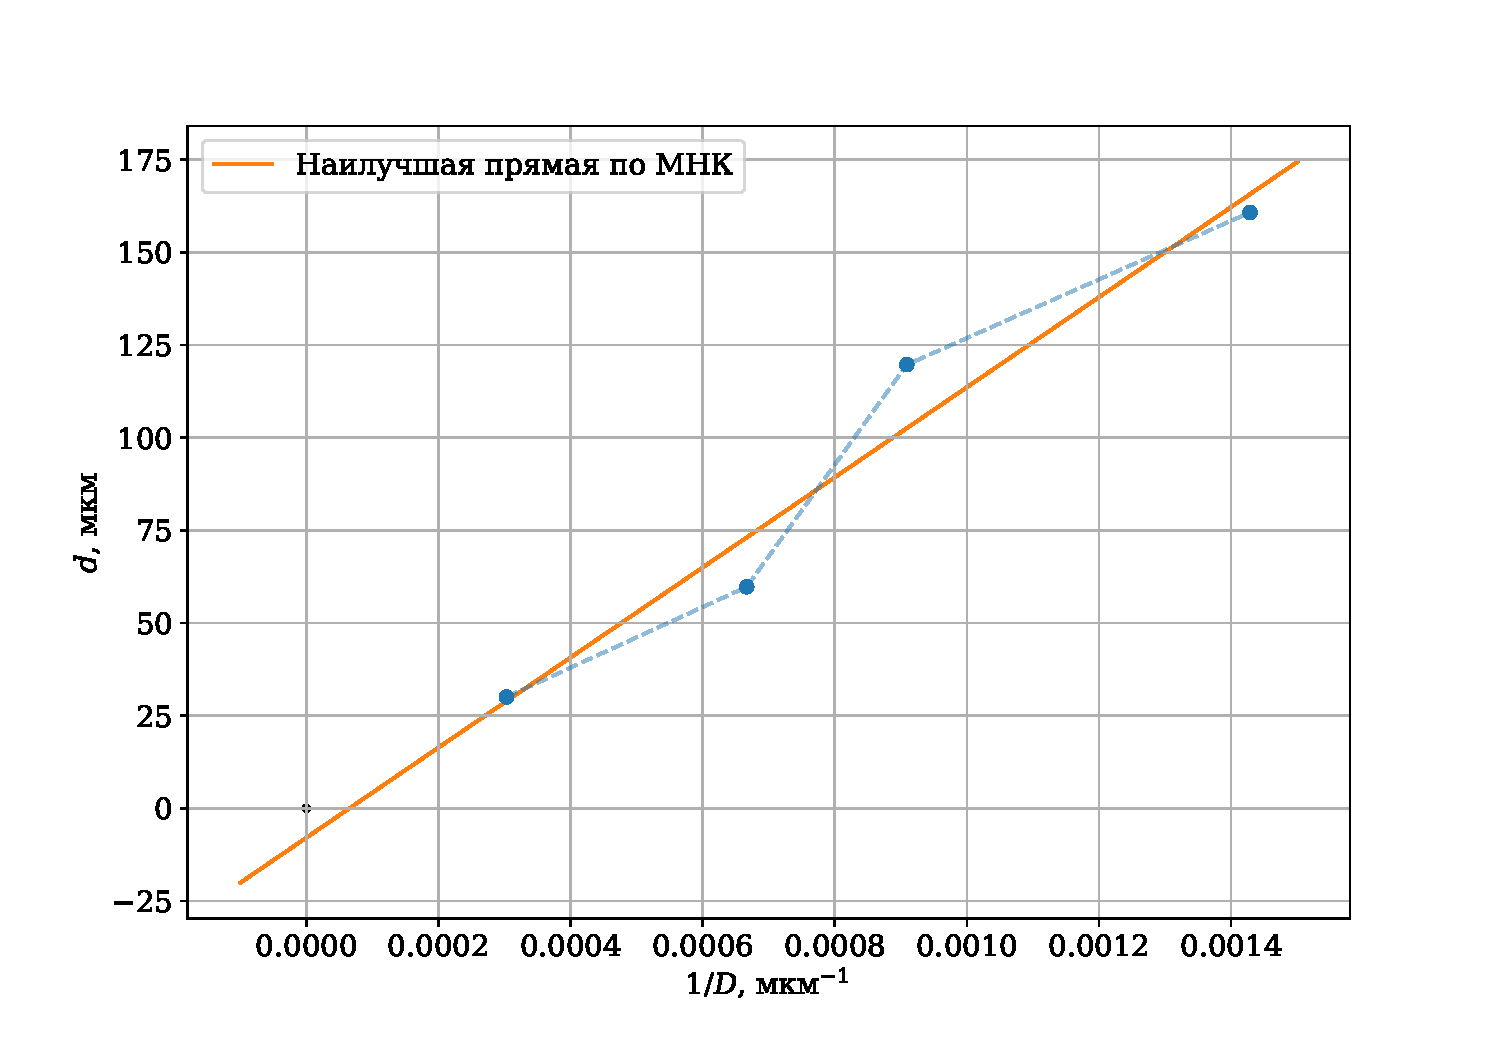
\includegraphics[width=\textwidth]{plot.pdf}
\caption{График зависимости $d = f(1/D)$}
\label{fig:plot}
\end{figure}

\subsection{Пространственная фильтрация и мультиплицирование}

\paragraph{Пространственная фильтрация.} Пропуская только вертикальные дифракционные максимумы, получим на экране картинку горизонтальных полос, находящихся на расстоянии равном увеличенному периоду решётки друг от друга. При пропускании только горизонтальных максимумов, получим такие же полосы, но расположенные вертикально.
\paragraph{} Пропуская только диагональные максимумы, получим изображение решётки с периодом, увеличенным в $\sqrt{2}$ раз. 

\paragraph{Мультиплицирование.} Расположив щель за дифракционной решёткой, получим множество изображений щелей, повторяющихся периодически по горизонтали и вертикали.

\medskip\hrule\medskip

\section{Выводы}

\begin{enumerate}
\item Нашли периоды дифракционных решёток тремя способами и получили следующие значения:

\begin{table}[h]
\centering
\begin{tabular}{|l|ll|ll|l|}
\hline
    & \multicolumn{2}{c|}{$I$ способ}                 & \multicolumn{2}{c|}{$II$ способ}                & \multicolumn{1}{c|}{$III$ способ} \\ \hline
$N$ & \multicolumn{1}{l|}{$d$, мкм} & $\sigma_d$, мкм & \multicolumn{1}{l|}{$d$, мкм} & $\sigma_d$, мкм & $d$, мкм                          \\ \hline
1 & \multicolumn{1}{l|}{19.90} & 0.30 & \multicolumn{1}{l|}{15.2} & 1.1 &     \\ \hline
2 & \multicolumn{1}{l|}{30.03} & 0.50 & \multicolumn{1}{l|}{22.4} & 1.6 & 35  \\ \hline
3 & \multicolumn{1}{l|}{59.8}  & 1.0  & \multicolumn{1}{l|}{69.7} & 5.0 & 78  \\ \hline
4 & \multicolumn{1}{l|}{119.7} & 2.2  & \multicolumn{1}{l|}{136}  & 11  & 106 \\ \hline
5 & \multicolumn{1}{l|}{160.8} & 2.6  & \multicolumn{1}{l|}{176}  & 14  & 167 \\ \hline
\end{tabular}
\caption{Периоды решёток, полученные разными способами}
\label{tab:mets}
\end{table}

\item Основываясь на полученных данных проверили теорию Аббе

\item Пронаблюдали качественно эффекты пространственной фильтрации и мультиплицирования.

\end{enumerate}



\end{document}
